% ──────────────────────────────────────────────────────────────────────────────
% Process-Driven Agentification — Verification of the Agentic Study Planner
% OvGU Workshop AgenticAI · June 2026 · Nandish Karki
%
% Compile:  pdflatex process_model_verification.tex
% Requires: tikz, booktabs, geometry, xcolor (all in TeX Live / MiKTeX base)
% ──────────────────────────────────────────────────────────────────────────────
\documentclass[11pt,a4paper]{article}
\usepackage[margin=2.5cm]{geometry}
\usepackage{tikz}
\usetikzlibrary{positioning,arrows.meta,calc}
\usepackage{booktabs}
\usepackage{xcolor}
\usepackage{array}
\usepackage[hidelinks]{hyperref}

\definecolor{stagefill}{RGB}{245,245,245}
\definecolor{okgreen}{RGB}{0,128,0}
\definecolor{partialorange}{RGB}{204,102,0}

\newcommand{\satisfied}{\textcolor{okgreen}{\textbf{Satisfied}}}
\newcommand{\partialk}{\textcolor{partialorange}{\textbf{Partial}}}

\title{Process-Driven Agentification:\\
       Verification of the \emph{Agentic Study Planner}}
\author{Nandish Karki \\ M.Sc.\ Data \& Knowledge Engineering, OvGU Magdeburg}
\date{June 2026}

\begin{document}
\maketitle

\section{The reference lifecycle}

The workshop's process-driven agentification methodology follows a six-stage
lifecycle: an \emph{as-is} process is modelled, analysed, and redesigned into a
\emph{to-be} model, which is then \emph{agentified} (mapped onto LLM agents),
evaluated by users, and monitored --- with performance insights feeding back
into the next analysis iteration.

\begin{figure}[h]
\centering
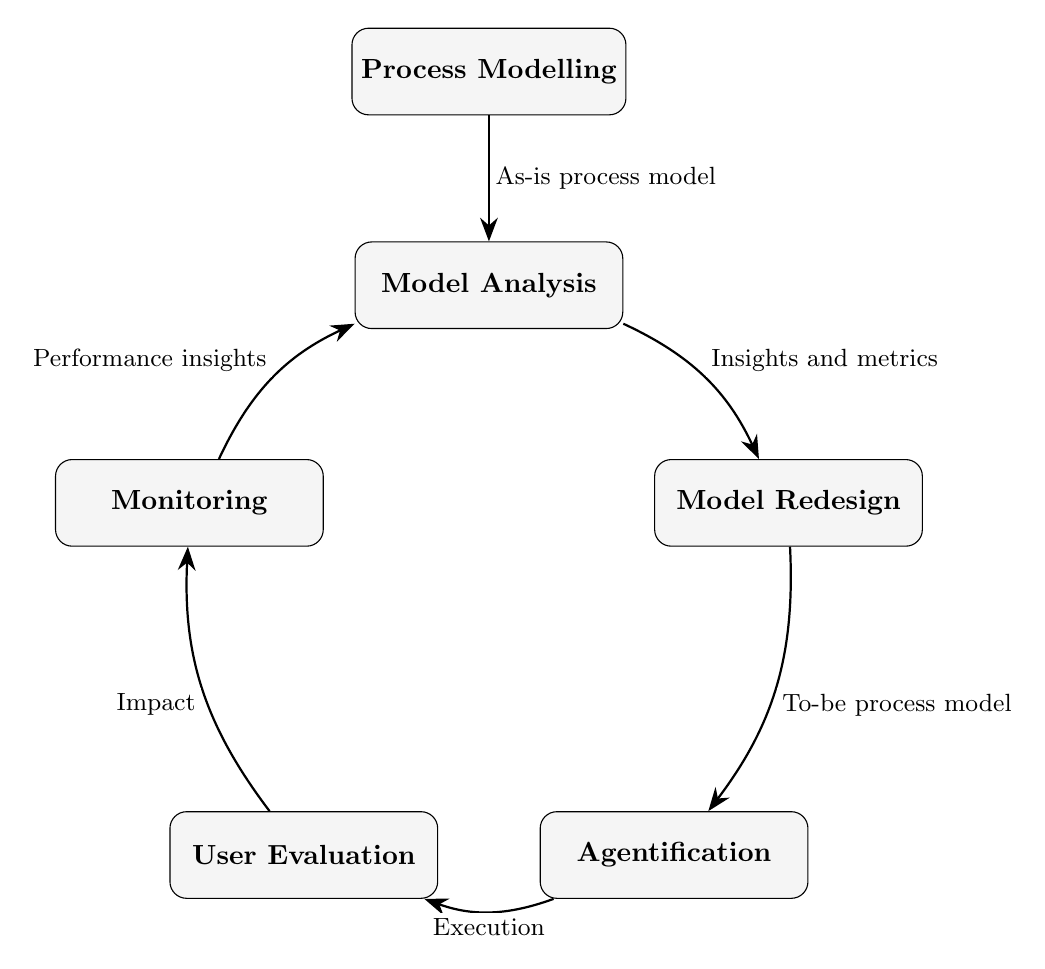
\begin{tikzpicture}[
    stage/.style={draw, rounded corners=6pt, fill=stagefill, minimum width=3.4cm,
                  minimum height=1.1cm, font=\bfseries, align=center},
    flow/.style={-{Stealth[length=3mm]}, thick},
    lab/.style={font=\small, fill=white, inner sep=2pt}
]
    % Cycle nodes on a circle of radius 4cm, Model Analysis at top (90°)
    \node[stage] (analysis)  at (90:4)   {Model Analysis};
    \node[stage] (redesign)  at (18:4)   {Model Redesign};
    \node[stage] (agentify)  at (-54:4)  {Agentification};
    \node[stage] (evaluate)  at (-126:4) {User Evaluation};
    \node[stage] (monitor)   at (162:4)  {Monitoring};

    % Entry node above the cycle
    \node[stage, above=1.6cm of analysis] (modelling) {Process Modelling};

    \draw[flow] (modelling) -- node[lab, right] {As-is process model} (analysis);

    \draw[flow] (analysis)  to[bend left=20]
        node[lab, above right] {Insights and metrics} (redesign);
    \draw[flow] (redesign)  to[bend left=20]
        node[lab, below right] {To-be process model} (agentify);
    \draw[flow] (agentify)  to[bend left=20]
        node[lab, below] {Execution} (evaluate);
    \draw[flow] (evaluate)  to[bend left=20]
        node[lab, below left] {Impact} (monitor);
    \draw[flow] (monitor)   to[bend left=20]
        node[lab, above left] {Performance insights} (analysis);
\end{tikzpicture}
\caption{The process-driven agentification lifecycle (workshop reference model).}
\label{fig:lifecycle}
\end{figure}

\section{Stage-by-stage verification}

\begin{table}[h]
\centering
\small
\begin{tabular}{@{}p{2.6cm}p{1.7cm}p{9.6cm}@{}}
\toprule
\textbf{Stage} & \textbf{Verdict} & \textbf{Evidence in the project} \\
\midrule
Process Modelling & \partialk &
The as-is process (a student manually cross-referencing CV, transcript,
career goal, and module handbook) is described in the README, but no formal
as-is model (e.g.\ BPMN) was produced. \\
\addlinespace
Model Analysis & \partialk &
Pain points were identified qualitatively (document-heavy, error-prone,
hallucination risk when an LLM plans unaided). No quantitative metrics of the
manual process (time, error rate) were collected. \\
\addlinespace
Model Redesign & \satisfied &
\texttt{config/tasks.yaml} \emph{is} the to-be process model: a declarative
task graph with explicit \texttt{context:} dependencies --- three parallel
analyses (profile, career, modules) feeding a two-stage synthesis (gap
analysis $\rightarrow$ semester plan). The README documents this dataflow. \\
\addlinespace
Agentification & \satisfied &
The model is mapped one-to-one onto a CrewAI crew:
\texttt{agents.yaml}/\texttt{tasks.yaml} define five agents and tasks;
document tools (\texttt{read\_document}, \texttt{search\_document}) ground the
analysts in real PDFs; the two synthesis agents are deliberately
\emph{tool-less} so they can only reason over upstream outputs (grounding by
construction); models are routed by capability (fast model for extraction,
strong model for synthesis). \\
\addlinespace
User Evaluation & \partialk &
One verified end-to-end run on real documents; the generated plan was read in
full and checked manually ($\sim$30 ECTS per semester, no invented modules,
prerequisites respected). However $n{=}1$ and the evaluator is the author ---
no independent users yet. \\
\addlinespace
Monitoring & \partialk &
The resolved LLM configuration is logged at startup, agent execution is
traced verbosely, and rate-limit retries are logged. No metrics are
\emph{persisted} (latency, tokens, grounding violations), so there is no
performance-insight feedback into a next analysis iteration. \\
\bottomrule
\end{tabular}
\caption{Verification of the Agentic Study Planner against the lifecycle.}
\label{tab:verification}
\end{table}

\section{Verdict}

The project \textbf{traverses the lifecycle once but does not yet close the
loop}. The forward path --- Modelling $\rightarrow$ Analysis $\rightarrow$
Redesign $\rightarrow$ Agentification --- is implemented, with the
Redesign and Agentification stages satisfied rigorously: the process model is
an explicit, declarative artifact (\texttt{tasks.yaml}) rather than prose, and
the agent mapping enforces grounding structurally (tool-less synthesis agents)
instead of relying on prompt instructions alone.

The backward path --- User Evaluation $\rightarrow$ Monitoring $\rightarrow$
Model Analysis --- exists only in embryonic form. Closing it requires
(i)~independent users executing the system and rating its impact, and
(ii)~persisted run metrics that can drive the next redesign. Both are planned:
the workshop distribution (other students testing the planner on their own
documents) directly implements the User Evaluation stage, and a metrics
sidecar per run implements Monitoring. See \texttt{FUTURE.md} in the
repository for the concrete roadmap.

\end{document}
